% This is "sig-alternate.tex" V2.0 May 2012
% This file should be compiled with V2.5 of "sig-alternate.cls" May 2012
%
% This example file demonstrates the use of the 'sig-alternate.cls'
% V2.5 LaTeX2e document class file. It is for those submitting
% articles to ACM Conference Proceedings WHO DO NOT WISH TO
% STRICTLY ADHERE TO THE SIGS (PUBS-BOARD-ENDORSED) STYLE.
% The 'sig-alternate.cls' file will produce a similar-looking,
% albeit, 'tighter' paper resulting in, invariably, fewer pages.
%
% ----------------------------------------------------------------------------------------------------------------
% This .tex file (and associated .cls V2.5) produces:
%       1) The Permission Statement
%       2) The Conference (location) Info information
%       3) The Copyright Line with ACM data
%       4) NO page numbers
%
% as against the acm_proc_article-sp.cls file which
% DOES NOT produce 1) thru' 3) above.
%
% Using 'sig-alternate.cls' you have control, however, from within
% the source .tex file, over both the CopyrightYear
% (defaulted to 200X) and the ACM Copyright Data
% (defaulted to X-XXXXX-XX-X/XX/XX).
% e.g.
% \CopyrightYear{2007} will cause 2007 to appear in the copyright line.
% \crdata{0-12345-67-8/90/12} will cause 0-12345-67-8/90/12 to appear in the copyright line.
%
% ---------------------------------------------------------------------------------------------------------------
% This .tex source is an example which *does* use
% the .bib file (from which the .bbl file % is produced).
% REMEMBER HOWEVER: After having produced the .bbl file,
% and prior to final submission, you *NEED* to 'insert'
% your .bbl file into your source .tex file so as to provide
% ONE 'self-contained' source file.
%
% ================= IF YOU HAVE QUESTIONS =======================
% Questions regarding the SIGS styles, SIGS policies and
% procedures, Conferences etc. should be sent to
% Adrienne Griscti (griscti@acm.org)
%
% Technical questions _only_ to
% Gerald Murray (murray@hq.acm.org)
% ===============================================================
%
% For tracking purposes - this is V2.0 - May 2012

\documentclass{sig-alternate}

\begin{document}
%
% --- Author Metadata here ---
\conferenceinfo{WOODSTOCK}{'97 El Paso, Texas USA}
%\CopyrightYear{2007} % Allows default copyright year (20XX) to be over-ridden - IF NEED BE.
%\crdata{0-12345-67-8/90/01}  % Allows default copyright data (0-89791-88-6/97/05) to be over-ridden - IF NEED BE.
% --- End of Author Metadata ---

\title{Energy Aggregation using Product of HMM}
%\title{Alternate {\ttlit ACM} SIG Proceedings Paper in LaTeX
%Format\titlenote{(Produces the permission block, and
%copyright information). For use with
%SIG-ALTERNATE.CLS. Supported by ACM.}}
%\subtitle{[Extended Abstract]
%\titlenote{A full version of this paper is available as
%\textit{Author's Guide to Preparing ACM SIG Proceedings Using
%\LaTeX$2_\epsilon$\ and BibTeX} at
%\texttt{www.acm.org/eaddress.htm}}}
%
% You need the command \numberofauthors to handle the 'placement
% and alignment' of the authors beneath the title.
%
% For aesthetic reasons, we recommend 'three authors at a time'
% i.e. three 'name/affiliation blocks' be placed beneath the title.
%
% NOTE: You are NOT restricted in how many 'rows' of
% "name/affiliations" may appear. We just ask that you restrict
% the number of 'columns' to three.
%
% Because of the available 'opening page real-estate'
% we ask you to refrain from putting more than six authors
% (two rows with three columns) beneath the article title.
% More than six makes the first-page appear very cluttered indeed.
%
% Use the \alignauthor commands to handle the names
% and affiliations for an 'aesthetic maximum' of six authors.
% Add names, affiliations, addresses for
% the seventh etc. author(s) as the argument for the
% \additionalauthors command.
% These 'additional authors' will be output/set for you
% without further effort on your part as the last section in
% the body of your article BEFORE References or any Appendices.

\numberofauthors{4} %  in this sample file, there are a *total*
% of EIGHT authors. SIX appear on the 'first-page' (for formatting
% reasons) and the remaining two appear in the \additionalauthors section.
%
\author{
% You can go ahead and credit any number of authors here,
% e.g. one 'row of three' or two rows (consisting of one row of three
% and a second row of one, two or three).
%
% The command \alignauthor (no curly braces needed) should
% precede each author name, affiliation/snail-mail address and
% e-mail address. Additionally, tag each line of
% affiliation/address with \affaddr, and tag the
% e-mail address with \email.
%
\alignauthor
Megha Gupta\\
       \affaddr{Department of Computer Science}\\
       \affaddr{IIIT Delhi, India}\\
       \email{meghag@iiitd.ac.in}
\alignauthor
Haimonti Dutta\titlenote{The author is also affiliated to the Institute of Data Science and Engineering (IDSE), Columbia University and is an adjunct professor at IIIT-Delhi.}\\
       \affaddr{Department of Management Science and Systems,}\\
       \affaddr{State University of New York, Buffalo}\\
       \affaddr{New York, 14260}\\
       \email{haimonti@buffalo.edu}
\alignauthor 
Ullas Nambiar\\
       \affaddr{EMC Corporation}\\
       \affaddr{Bangalore, India}\\
       \email{ullas.nambiar@emc.com}
\and  % use '\and' if you need 'another row' of author names
\alignauthor Amarjeet Singh \\
       \affaddr{Department of Computer Science}\\
       \affaddr{IIIT Delhi}\\
       \email{amarjeet@iiitd.ac.in}
}

% There's nothing stopping you putting the seventh, eighth, etc.
% author on the opening page (as the 'third row') but we ask,
% for aesthetic reasons that you place these 'additional authors'
% in the \additional authors block, viz.
%\additionalauthors{Additional authors: John Smith (The Th{\o}rv{\"a}ld Group,
%email: {\texttt{jsmith@affiliation.org}}) and Julius P.~Kumquat
%(The Kumquat Consortium, email: {\texttt{jpkumquat@consortium.net}}).}
%\date{30 July 1999}
% Just remember to make sure that the TOTAL number of authors
% is the number that will appear on the first page PLUS the
% number that will appear in the \additionalauthors section.

\maketitle
\begin{abstract}
The need to gather real-time fine grained spatio-temporal energy consumption data is fulfilled by the large scale deployment of smart meters. With the advent of smart metering infrastructure in the electrical power systems, remote monitoring is done by sending the readings from the customer's place to the data aggregators placed at the substations. Each substation aggregates the load derived from all the meters connected to that substation. The problem arises when the analytics is to be performed on the data which is aggregated from the inconsistent messages passed by all the meters connected to a particular substation.
%the demand response programs have been a cost effective alternative to meet the occasional peak demands. 
We propose to solve the problem of energy aggregation where the constituents of each aggregate are inconsistent with respect to time. The challenges with the inconsistent data includes aggregating non-aligned time stamped readings, readings with missing values, repeated values, meter reset readings. We address the problem of aggregating energy data in context with the load forecasting using an ensemble based learning technique called product of Hidden Markov Models (PoHMM). The objective function used for learning here is the contrastive divergence between the observed data and the reconstructed data produced by running a Gibbs sampler. 
%Data analytics in energy domain, load forecasting on aggregates of power meters, Energy aggregation problem using pohmm, The STLF accuracy improves with larger aggregates, This paper deals with the energy aggregation problems in electrical system. The challenges included problem of aggregating inconsistent data, across time, in case of electrical systems.



%This paper provides a sample of a \LaTeX\ document which conforms,
%somewhat loosely, to the formatting guidelines for
%ACM SIG Proceedings. It is an {\em alternate} style which produces
%a {\em tighter-looking} paper and was designed in response to
%concerns expressed, by authors, over page-budgets.
%It complements the document \textit{Author's (Alternate) Guide to
%Preparing ACM SIG Proceedings Using \LaTeX$2_\epsilon$\ and Bib\TeX}.
%This source file has been written with the intention of being
%compiled under \LaTeX$2_\epsilon$\ and BibTeX.
%
%The developers have tried to include every imaginable sort
%of ``bells and whistles", such as a subtitle, footnotes on
%title, subtitle and authors, as well as in the text, and
%every optional component (e.g. Acknowledgments, Additional
%Authors, Appendices), not to mention examples of
%equations, theorems, tables and figures.
%
%To make best use of this sample document, run it through \LaTeX\
%and BibTeX, and compare this source code with the printed
%output produced by the dvi file. A compiled PDF version
%is available on the web page to help you with the
%`look and feel'.
\end{abstract}

%% A category with the (minimum) three required fields
%\category{G.3}{Mathematics of Computing}{Probability and Statistics- Time Series Analysis }
%%A category including the fourth, optional field follows...
%\category{D.2.8}{Software Engineering}{Metrics}[complexity measures, performance measures]
%
%\terms{Theory}

\keywords{Energy aggregation; Ensemble learning; Product of HMM }

\section{Introduction}
Smart meters consisting of real time sensors, power outage notifications and power quality monitoring are widely used today. These meters provide a host of benefits like energy efficiency and savings, improved retail competition, better demand response actions, improved tariffs, lower bills due to better customer feedback, accurate billing, less environmental pollution, etc. %\cite
They generate huge amount of data which helps in giving meaningful insights through analytics.
They can measure site specific information and also help agencies to set different electricity prices for consumption based on the time of the day, seasons, holidays, etc. As a result, a feedback is sent to the customers by the utilities that can help consumers better manage their resources. A research \cite{mckerracher} shows that by providing real time feedback, consumers can reduce the consumption by 3-5\%. Also, for some country providing real time feedback may not be a cost effective plan but it can help in retaining customers and peak-load shift.
%This helps consumers to better manage their energy resources and reduce their bills and carbon emissions.


In recent years, machine learning has been applied to the problem of energy consumption and demand forecasting analysis. The role of the machine learning algorithm is to study the sensor data and provide alerts and warnings when anomalous behaviour occurs or to inform (and remind) customers when certain activities were performed, which rooms they occupied, and what appliances they used most frequently during that period. This information can be transmitted to customers in timely fashion via phone, email or the Internet.
This paper \cite{1626400} does a comparison of several clustering techniques and finds out that  the hierarchical clustering and modified follow-the-leader perform best among the rest K-Means, fuzzy K-Means to group customers with similar electrical behaviour \cite{5620917}. Another paper \cite{Wijaya} uses classifiers like random forest, J48, logistic and naive bayes to identify customers with similar electricity consumption profiles.
Sensor data collected from smart homes are used to reveal activity patterns of the residents, which can then be correlated with the total energy consumption. This enables utility companies and their customers to associate activities with energy usage and costs, devise intelligent systems to control home environments improving energy efficiency and reducing costs. Typically, sequences of usage patterns that appear frequently at different time scales (daily, weekly, monthly, yearly) and across different homes are studied and 
%; trends of electricity consumption (steadily increasing, decreasing, cyclic, seasonal) for individual homes and across the community; and anomalies (sudden peaks or drops on consumption) for individual homes and across the community.
outlier detection algorithms are designed to enable customers to be notified that they are consuming unusually large amount(s) of energy during some specific period. Related problems involve study of trends of electricity consumption (steadily increasing, decreasing, cyclic, seasonal) and sudden anomalous behaviour (sudden peaks or drops on consumption) for individual homes and across the community.

In this paper, we use HMMs to model time series data. We build machine learning models using products of HMMs and apply them to the energy aggregation problem. Two different proof of concepts are presented -- first one on the REDD data set and the other one on real data collected at the faculty housing in India. 
%application of are aggregating energy consumption information using a model that extends the power of HMMs. HMM's are used as the basic expert in the of product of experts model. 
There are many reasons why the product model constructed from many HMMs is appropriate. First, this model is ideal for data which is caused by multiple underlying influences. Second, HMMs alone are not efficient at capturing long range structure in time series \cite{Taylor} -- in contrast to product of hidden markov models (PoHMM)  \cite{andrew} allow each model to remember a different piece of information about the past.
%There have been some experiments on sentence and character strings modelling, factorial time series to demonstrate the advantages of using a PoHMM over an equivalently sized regular HMM}.
%We have applied the contrastive divergence learning algorithm on two datasets, REDD dataset and the faculty housing dataset which was generated by smart meters.
%The system architecture for the faculty housing dataset consists of two smart meters $S_1$ and $S_2$ installed in a faculty housing building collecting data from twelve floors. $S_1$ collects data from first six floors (0 to 5th) and $S_2$ collects data from the rest of the floors (6 to 11th). The data collected from two meters is aggregated using product of experts technique in a way that the contrastive divergence between the two probability distributions is minimized. 
%The proof of concept of REDD dataset and faculty housing dataset is given in section~\ref{sec:redd} and section~\ref{sec:faculty} respectively.

\noindent \textbf{Organization:} This paper is organized as follows: Section~\ref{related} examines related work on data analytics on aggregated data of smart meters; Section~\ref{sec:review} provides a review of products of Hidden Markov Models (HMMs) and how they relate to our application. The two proofs of concepts are introduced in Section~\ref{poc} to illustrate the effectiveness of the use of product of HMMs in the energy aggregation problem. Finally, Section~\ref{conc} concludes the work.

\section{Related Work}
\label{related}
In this section, we describe work that uses ensemble learning techniques and non-ensemble learning techniques to solve problems in energy domain.
\subsection{Non-ensemble based learning techniques}

\subsubsection{Energy Aggregation}
%Devaine et al. (CITE) study ...
In wireless sensor networks, energy data aggregation is a method of combining data from different sources and expressing on a specific variable, in a summarised format. As the sensor network generates lot of data for the end user to process, there are automated methods employed to aggregate data. This data fusion is generally known as data aggregation which combines the data into a set of meaningful information \cite{Heinzelman00energy}.
The sensor nodes are organised in a tree structure, called aggregation tree. The leaves of this tree are the sensor devices, the internal nodes are the aggregator devices that takes the data from the leaves, aggregates it and sends it to its parent node which is the root of the tree. \\
The main objective of data aggregation is to reduce the unnecessary information thereby reducing the network traffic and improving the privacy of the customers from internal and external entities by keeping only the necessary information \cite{taban}. 


%To study the process of energy aggregation, data is collected from multiple smart meters. This collected data is very large which in turn makes the analytics on top of it very difficult. Also, this detailed energy consumption data leads to privacy breach and other risks related to it. To address this problem, there has been work done \cite{Wijaya} to reduce the smart meter data numerosity by converting it into symbolic representation and then allowing algorithms on top of it. They have applied the symbolic representation tasks for customer segmentation and load forecasting.

%The purpose of energy aggregation is to get some valuable information about single or multi-site units. 
%This work evaluates the trend of degrading performance of the state of the art algorithms when the number of considered meters decrease \cite{BLTJ:BLTJ21650}. Short term load forecasts at the meter level help the company communicate with the customer about energy savings and billing. STLF handles prediction of one hour upto one week.
%The energy aggregation problem has been tackled in a variety of ways including topology control, energy conserving sleep scheduling, mobile data collectors and data aggregation. 
%Research has been done on the role of energy on the growth of the country's economy \cite{NYAS:NYAS5921}.

\subsubsection{Energy Disaggregation}
The process in which the whole building energy (aggregated) signal is separated into appliance level energy (disaggregated) for a variety of reasons like residential energy reductions, program evaluation, targeted marketing, etc. Several studies have been done in this regard, one of the unsupervised desegregation method \cite{DisaggregationHSMM} that outperforms other unsupervised disaggregation methods is conditional factorial hidden semi-Markov model. This model when integrated with other features, accurately represents the individual appliance energy consumption. Another research \cite{KolterJ12} that exploits the additive structure of the FHMM to develop approximate inference procedure in  energy disaggregation domain that outperforms the rest.

\subsubsection{Load Forecasting}
Electrical load forecasting refers to the projection of electrical load required in a certain geographical area with the use of previous electrical load usage in the same area. It is extremely important for efficient power system planning and operation, energy purchasing and generation, load switching, infrastructure development. It encompasses various factors like, historical load, weather data, population, energy supply and price, time of the year, etc.
It is usually divided into three categories, short-term forecasts (one hour to one week) , medium-term forecasts (one week to one year) and long-term forecasts (more than a year).
In short term load forecast, \cite{Bakirtzis} and \cite{Chen} used a three layer feed forward artificial neural network and to predict daily load profiles. In a paper by \cite{Chow}, nonlinear autoregressive integrated neural network was used to predict daily load consumption.
In medium term load forecasts, the author forecasts \cite{Falvo} the monthly load through knowledge based activities from the output of the ANN based stage providing yearly energy predictions. Whereas in \cite{bassi}, time lagged feedforward neural network is used to do monthly forecasting on the basis of historical series of electrical load, economic and demographic variables. And the authors from covenant university, \cite{samuel} performed load forecasting of their own educational institute using the models based on linear, compound growth and cubic methods of regression analysis.
In long term load forecasting, study done by \cite{Daneshi} resulted in showing that the models based on regression analysis did not give very accurate predictions as compared to fuzzy neural network which performed better due to better handling with non linear systems. Another work  \cite{Zhang} uses support vector regression to derive non linear relationship between load and economic factors like GDP for long term forecasting in developing countries.



\subsubsection{Customer Segmentation}
The identification of consumer profiles that show similar behaviour in energy consumption. This analysis is useful in various ways, like demand response system, intelligent distribution channel. The author \cite{wijaya2014consumer} segments the customers based on contextual dimensions like location, seasons, weather patterns, holidays, etc which help with various higher level applications like usage-specific tariff structure, theft detection, etc. In \cite{Albert}, author proposes to infer occupancy states from consumption time series data by using HMM framework. They investigate the effectiveness of HMM and model based cluster analysis in producing meaningful features of the classification. This work suggests the dynamics of time series as captured by HMM analysis can be valuable.

\subsection{Ensemble based learning techniques}
Ensemble learning is a method where multiple learners are trained to solve the same problem. It constructs a set of hypothesis and combines them to generate the final result.
\subsubsection{Prediction with expert advice}
A study done by \cite{Shen}, proposes a Pattern Forecasting Ensemble Model (PFEM) comprising of five forecasting models using different clustering techniques, like k-means model, self-organising map model, hierarchical clustering model, k-medoids model and fuzzy c-means model. They have showed that on three real-world dataset, their proposed ensemble model outperformed all the five individual model in case of day ahead electricity demand prediction.
Another study \cite{Felice} highlights the importance of regularised negative correlation learning ensemble methodology on the problem of energy load hourly prediction. This method tries to overcomes the problem of variability in neural network due to high sensitivitiness to the initial conditions. As this method combines the outputs of several neural networks, it achieves a marked reduction in error after introducing external data. \\
In our paper,  we deal with the problem of energy aggregation using ensemble learning model. Each HMM is used to represent a state of an appliance. An appliance can have states like ON or OFF. The combination of the outputs from each of these HMM models gives us our ensemble based learning model, Product of Hidden Markov Model (PoHMM) \cite{hinton2000}. This learning technique outputs the probability distribution by combining the outputs from several simpler distributions. It allows each model to make a decision on the basis of few dimensions.


\section{Review of PoHMM}
\label{sec:review}
%Benveniste defines HMM as a triple (\'{A}, $\mu$, $\pi$) where \'{A} = (X,$X_0$,A,T) is an automaton, $\mu$ is the initial state probability, $\pi$ is factored as state transition probability $\pi$$_{x}$ and message transition probability $\pi$$_{A}$. He uses a random arbiter $\alpha$, with values {first, second, third} to choose automaton to initiate transition. If $\alpha$ = first then first automaton chooses any transition having a private message whereas second automaton performs a stuttering transition, and vice versa for $\alpha$ = second. If $\alpha$ = both, then both automata agree on some shared message and move accordingly.

A hidden Markov Model (HMM) is a tool that represents the probability distribution over the sequence of observations \cite{Ghahramani}. It holds two name defining properties, first, the observation at time $t$ is generated by a process whose state $S_{t}$ is hidden from the observer and second, is that this hidden state process satisfies Markov property which states that given the value at state $S_{t-1}$, the value at current state $S_{t}$ is independent of all the states prior to $t-1$. Another assumption that it follows is that the hidden state variable is discreet, that is $S_{t}$ can take $K$ values denoted by integers \{1,..K\}. In order to define probably distribution  over the sequence of observation, it is important to define probability distribution over the initial state P($S_{1}$), the transition probability P($S_{t}$|$S_{t-1}$) and the observed probability P($Y_{t}$|$S_{t}$) where $Y_{t}$ is the observation at time $t$.
%HMMs are widely used for modelling time series data. They are found useful in applications like speech, handwriting, gesture recognition, part-of-speech tagging, bioinformatics, etc.

Using the traditional HMM notation for the parameter $\lambda$ = \{A, B, $\pi$ \} where A is the transition probability, B is the observed probability and $\pi$ is the initial state probability. For HMMs, $S^{1}$ \& $S^{2}$ we have the values of A, B, $\pi$ as shown in table ~\ref{table:A}, ~\ref{table:B}, ~\ref{table:pi} respectively.

%Distributed networks can be modeled using interacting automata.
%Benveniste \cite{benveniste} defines automaton as a quadruple, \'{A} = (X,$X_0$,A,T) where X is a finite state of sets, $X_0$ is the subset of initial states, A is a finite set of messages, T is a set of transitions of the form t = \{x\_,a,x\} where x\_ is the previous state, a is the message label on which the state transitions to the next state x. The figure~\ref{fig:ex} below explains the automata with an example.\\

%\begin{figure*}[t]
%\centering
%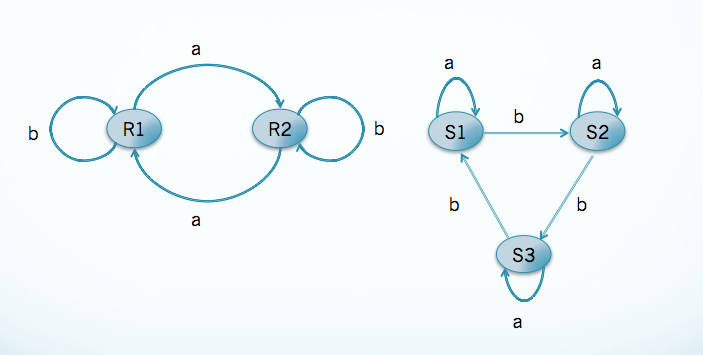
\includegraphics[width=8cm,height=3cm]{automata.png}
%\caption{HMM R and S}
%\label{fig:ex}
%\end{figure*}

%For HMM R, X$_{R}$ = \{2; $R_1$,$R_2$\}, X$_{0R}$ = \{$R_1$\}, A$_{R}$ = \{a,b\}, T$_{R}$ = \{$R_1$,a,$R_1$; $R_1$,b,$R_2$; $R_2$,a,$R_2$; $R_2$,b,$R_1$\} \\
%For HMM S, X$_{S}$ = \{3; $S_1$,$S_2$,$S_3$\}, X$_{0S}$ = \{$S_1$\}, A$_{S}$ = \{a,b\}, T$_{S}$ = \{$S_1$,a,$S_1$; $S_1$,b,$S_2$; $S_2$,a,$S_2$; $S_2$,b,$S_3$; $S_3$,a,$S_3$; $S_3$,b,$S_1$\} \\
%The product of two HMMs P = R x S is defined as follows: \\
%X = X$_{R}$ x X$_{S}$ \\
%$X_0$ = X$_{0R}$ x X$_{0S}$ \\
%A = A$_{R}$ $\cup$ A$_{S}$ \\
%t = (x\_,a,x)  \\

%Benveniste uses a notion of stuttering transition which helps to distinguish between local and global time by inserting dummy transitions between two transitions of a local automaton attached to a node. This stuttering transition waits for others to progress.

\begin{table}[h]
\centering
\begin{tabular}{ l | c | c }
 $A_{S^{1}}$ & $S^1_1$ & $S^1_2$ \\
\hline
$R_1$ & 0.6 & 0.4 \\
$R_2$ & 0.3 & 0.7 \\
\end{tabular}
\quad
\begin{tabular}{ l | c | c | c }
  $A_{S^{2}}$ & $S^2_1$ & $S^2_2$ & $S^2_3$ \\
\hline
$S_1$ & 0.6 & 0.3 & 0.1 \\
$S_2$ & 0.4 & 0.1 & 0.5 \\
$S_3$ & 0.2 & 0.4 & 0.4 \\
\end{tabular}
\caption{Transition probabilities, A}
\label{table:A}
\end{table}

\begin{table}[h]
\centering
\begin{tabular}{ l | c | c }
 $B_{S^{1}}$ & a & b \\
\hline
$S^1_1$ & 0.2 & 0.8 \\
$S^1_2$ & 0.5 & 0.5 \\
\end{tabular}
\quad
\begin{tabular}{ l | c | c | c}
 $B_{S^{2}}$ & a & b & c\\
\hline
$S^2_1$ & 0.2 & 0.3 & 0.5 \\
$S^2_2$ & 0.5 & 0.4 & 0.1 \\
$S^2_3$ & 0.4 & 0.3 & 0.3 \\
\end{tabular}
\caption{Observed probabilities, B}
\label{table:B}
\end{table}

\begin{table}[h]
\centering
\begin{tabular}{ l | c | c }
&  $R_1$ & $R_2$ \\
\hline
$\pi_{S^{1}}$ & 0.4 & 0.6 \\
\end{tabular}
\quad
\begin{tabular}{ l | c | c | c}
&  $S_1$ & $S_2$ & $S_3$\\
\hline
$\pi_{S^{2}}$ & 0.4 & 0.4 & 0.2 \\
\end{tabular}
\caption{Initial state probabilities, $\pi$}
\label{table:pi}
\end{table}

%Talking in terms of HMM, requires us to equip products of automata with probabilities. 

\subsection{Product of HMM}
\label {sec:pohmm}
PoHMM is a way of combining multiple HMMs by multiplying their individual distribution together and then renormalizing them. Its representation includes both directed and undirected links where the hidden states are causally connected to the other hidden states but non causally related to the visible states. This causes different conditional independence relationships among the variables in graphical model. 
%It is a way of combining HMM's to form distributed state time series model. It is defined by multiplying together the densities of its, k experts and renormalizing them. 
The figure~\ref{fig:pohmm} is a product of two HMMs shown in~\ref{fig:ex}. For  P = $S^1$ x $S^2$, the number of states is the product of states in $S^1$ and $S^2$ which is 6. The connections formed in the P depend on the links in the multiplying HMMs. The resultant HMM will have a pair (s,s)
X = \{6; $R_1$$S_1$, $R_1$$S_2$, $R_1$$S_3$, $R_2$$S_1$, $R_2$$S_2$, $R_2$$S_3$\} \\
$X_0$ = \{$R_1$$S_1$\} \\
A = \{a,b\} \\
%The rules for synchronised product construction are : \\
%1. $<p,q>$ --a--$>$ $<p',q>$ if a $\in$ A$_{R}$ $\cap$ A$_{S}$ and p --a--$>$ p' and q --a--$>$ q'	\\
%2. $<p,q>$ --a--$>$ $<p',q>$ if a $\in$ A$_{R}$, a $\notin$ A$_{S}$ and p --a--$>$ p'	\\
%3. $<p,q>$ --a--$>$ $<p,q'>$ if a $\notin$ A$_{R}$, a $\in$ A$_{S}$ and q --a--$>$ q'	\\

%\begin{figure*}[t]
%\centering
%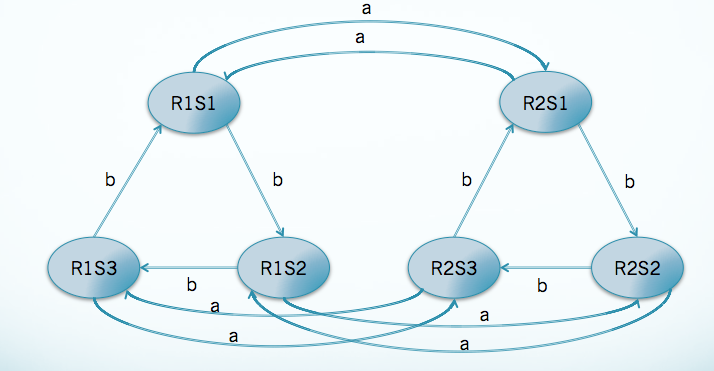
\includegraphics[width=8cm,height=3cm]{product.png}
%\caption{Product of HMMs, P = R x S}
%\label{fig:pohmm}
%\end{figure*}

%\section{ Methodology }
%\label{sec:method}
\subsection{Inference in PoHMM}

The main feature of PoE is its undirected graphical modelling with no direct connection among the latent variables as they only interact indirectly via observed variables. The hidden variables all the experts are rendered independent when conditioned on visible variables. So, if the inference in each of the constituent model is tractable then the inference in the product is also tractable. To generate a data point in this model, all the experts in PoE generate an observation and if they all generated the same point then it is accepted else they again generate an observation until all the experts agree to it. Therefore all the experts have some influence over the generated data. So, the inference determines the the probability that all the experts would have taken in order to generate the given observation. 

\begin{figure*}[t]
\centering
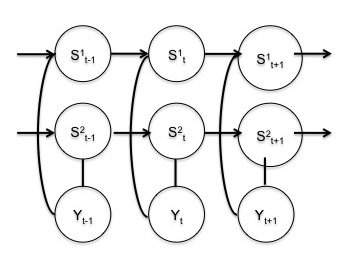
\includegraphics[width=5cm,height=3cm]{pohmm1.jpg}
\caption{Product of HMMs, P = $S^{1}$ x $S^2$}
\label{fig:PoHMM}
\end{figure*}

 
\subsection{Training product of experts by minimising contrastive divergence}
PoE is a method of combining densities of many latent variable models. It is defined by the following formula:\\
% Write the formula and explain it. Explain Gibbs Sampling
To fit the model to the data, we need to maximize the likelihood of the dataset or minimise the Kullback-Liebler divergence between the real data and the fantasy data. The contrastive divergence algorithm for training the PoHMM has the following steps:
\begin{enumerate}
\item Calculate each model's gradient on a data point using forward backward algorithm.
\item For each model take a sample from the posterior distribution of paths through state space.
\item At each time step, multiply together the distributions and renormalize to get the reconstruction distribution at each step.
\item Draw a sample from the reconstruction distribution at each time step to get a reconstructed sequence. Compute each model's gradient on the new sequence.
\item Update the parameters

\end{enumerate}
%High dimensional distributions are approximated as a product of one dimensional distributions. The product of individual distributions which are uniguassian or multivariate guassian will also be multivariate guassian. If the individual models are more complicated and contain one or more hidden variables, multiplying their distributions together and renormalizing them can be very powerful. These individual models are called "experts".
%The product of experts produce sharper distribution than the individual distributions\cite{hinton2000}.

\section{Proof of Concepts}
\label{poc}

\subsection{REDD House 2}
\label{sec:redd}
%\begin{enumerate}
\subsection{Aim}
 To represent streams of energy consumption data from $n$\footnote{n=2} appliances by product of $k$ HMMs.

\subsection{Method} 
\begin{itemize}
\item \textbf{Data } The Reference Energy Disaggregation Data Set (REDD) is used in empirical analysis. The data contains power consumption from real homes, for the whole house as well as for each individual circuit in
the house (labeled by the main type of appliance on that circuit). It is intended for use in developing disaggregation methods, which can predict, from only the whole-home signal, which devices are being used. The REDD data set contains two main types of home electricity data: high-frequency current/voltage waveform data of the two power mains (as well as the voltage signal for a single phase), and lower-frequency power data including the mains and individual, labeled circuits in the house. The main directory consists of several house directories, each of which contain all the power readings for a single house.  Each house subdirectory consists of a labels and channels files. The labels file contains channel numbers and a text label indicating the general category of device on this channel. Each channel\_i.dat file has two columns containing UTC timestamps (as integers) and power readings (recording the apparent power of the circuit) for the channel.
Experiments reported here use the House 2 data from REDD. It has $11$ channels where each channel corresponds to the following appliance: 
\begin{enumerate}
\item mains$\_1$ 
\item mains$\_2$ 
\item kitchen$\_$1
\item lighting
\item stove 
\item microwave
\item washer$\_$dryer
\item kitchen$\_2$
\item refrigerator
\item dishwaser
\item disposal
\end{enumerate}

The dataset has $318759$ records and $2$ columns. We randomly sample 300 records for our initial experiment. Time series data from two appliances are represented as product of $k$ HMMs.

\item \textbf{ Time Series :} The time series data of the microwave, dryer, kitchen$\_2$ and refrigerator are plotted below in Figures~\ref{fig:micro}, ~\ref{fig:washer}, ~\ref{fig:kitchen2}, ~\ref{fig:refri}.

\begin{figure*}[t]
\centering
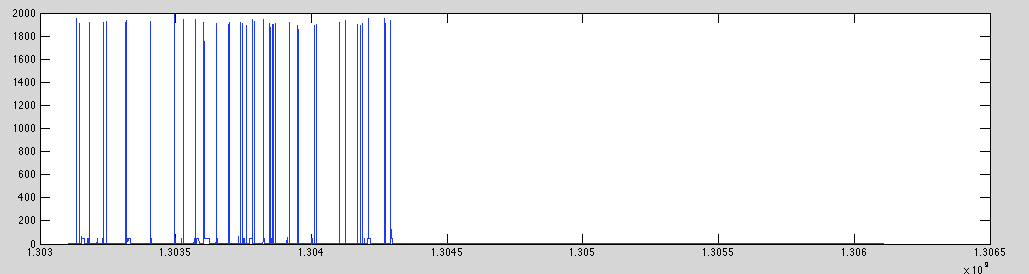
\includegraphics[width=1.0\textwidth,height=0.15\textheight]{channel_6.png}
\caption{Microwave}
\label{fig:micro}
\end{figure*}

\begin{figure*}[t]
\centering
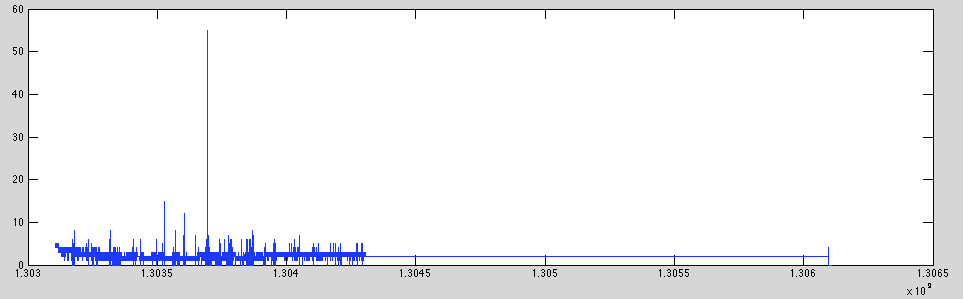
\includegraphics[width=1.0\textwidth,height=0.15\textheight]{channel_7.png}
\caption{washer\_dryer}
\label{fig:washer}
\end{figure*}

\begin{figure*}[th]
\centering
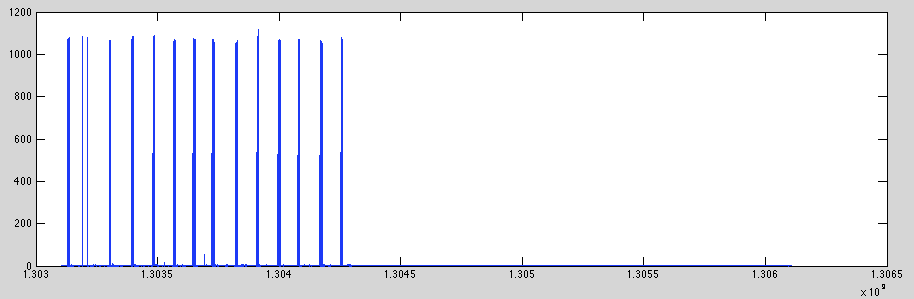
\includegraphics[width=1.0\textwidth,height=0.15\textheight]{channel_8.png}
\caption{Kitchen\_2}
\label{fig:kitchen2}
\end{figure*}

\begin{figure*}[th]
\centering
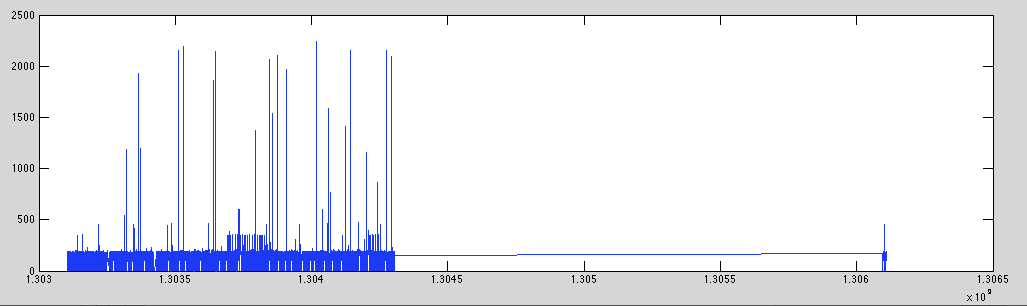
\includegraphics[width=1.0\textwidth,height=0.15\textheight]{channel_9.png}
\caption{refrigerator}
\label{fig:refri}
\end{figure*}

\item \textbf{Code } The implementation of the product of experts model is obtained from Iain Murray's website\footnote{\label{link}http://homepages.inf.ed.ac.uk/imurray2/code/}. It implements the technique described in Geoff Hinton's paper \cite{hinton2000}. 

\item \textbf{Additional details }
Some additional details regarding experiments:
\begin{enumerate}
\item The product of HMMs model (PoHMM) minimizes ``contrastive divergence" as described in the paper \cite{hinton2000}. 
\item The number of experts, $k$ used here is 15. This is set somewhat arbitrarily and needs to be experimented on.
\item Learning rate is $\epsilon = \frac{1}{300}$.
\end{enumerate}
 
\end{itemize}


%FIRST EXPERIMENT ON REDD DATASET

\subsection{Experimental Setup for REDD house 2}
Experiments are performed on the REDD which contains $9$ appliances each containing $318759$ rows of energy consumption data. Experiments are done into $4$ phases, in the first phase the number of data samples are varied corresponding to which the values of KL Divergence and convergence time are noted. In the second phase, the number of experts are varied keeping the best value of the sample from the first phase fixed. In the third phase, number of iterations are varied keeping the best values from above first two phases fixed. In the fourth part, the no. of appliances to be aggregated are varied.

\begin{table}[htdp]
\begin{center}
\begin{tabular}{| c | c | c | c |}
\hline
Samples & $KL Div$ & $T(sec)$ & $Iterations$ \\
\hline
300 & 2.4864 & 186.212 $\pm$9.087 & 18600 \\
500 & 0.6761 & 106.564 $\pm$10.046 & 10200 \\
1000 & 1.1088 & 158.521 $\pm$1.97  & 11200 \\
1500 & 3.8829 & 92.896 $\pm$8.075  & 5300 \\
2000 & 1.8686 & 130.98 $\pm$1.932 & 6900 \\
2500 & 0.4733 & 215.563 $\pm$ 2.471 & 9900 \\
3000 & 2.8204 & 258.213 $\pm1.918$ & 11000 \\
3500 & 1.2332 & 204.661 $\pm$1.713 & 7900 \\
4000 & 0.8959 & 292.666 $\pm$0.619 & 10400  \\
4500 & 1.1118 & 222.558 $\pm$1.967 & 7200  \\
8000 & 6.392 & 381.635 $\pm$2.952 & 8100  \\
10000 & 8.276 & 887.932 $\pm$13.824 & 10500  \\
15000 & 0.7201 & 1368.514 $\pm$13.605 & 9400  \\
\hline
\end{tabular}
\end{center}
\caption{Effect of varying samples on KL div and time}
\label{table: error1}
\end{table}

\begin{table}[htdp]
\begin{center}
\begin{tabular}{| c | c | c | c |}
\hline
Experts & $KL Div$ & $T(sec)$ & $Iterations$ \\
\hline
5 & 0.774 & 72.968 $\pm$1.177 & 5200 \\
10 & 1.424 & 117.482 $\pm$1.966 & 6700 \\
15 & 0.473 & 210.249 $\pm$1.258  & 9900 \\
20 & 1.56 & 217.739 $\pm$10.452 & 9000 \\
25 & 7.469 & 347.019 $\pm$8.23 & 12100 \\
30 & 2.4968 & 413.802 $\pm$7.304 & 12900 \\
35 & 1.5012 & 348.906 $\pm$14.651 & 11300 \\
\hline
\end{tabular}
\end{center}
\caption{Effect of varying experts on KL div and time}
\label{table: error2}
\end{table}


\subsection{Results}
The evaluation of how well the learning has taken place is done by using a Kullback-Leibler divergence. KL divergence of P from Q, $D_{KL}$(P$\parallel$Q) is the measure of information lost when Q is used to approximate P. Here, P is the real data and Q is a fantasy data. The two probability distributions in the REDD example refer to the expert probabilities in real and fantasy data. The learned parameters from the training are fitted to the fantasy data to measure the information lost when fantasy data is used to approximate real data.
\begin{table}[htdp]
\begin{center}
\begin{tabular}{| c | c | c | c |}
\hline
Threshold & $KL Div$ & $T(sec)$ & $Iterations$ \\
\hline
.1 & 0.473 & 210.6 $\pm$1.493 & 9900 \\
.05 & 0.443 & 240.607$\pm$2.436 & 10900 \\
.01 & 0.454 & 431.536 $\pm$14.509 & 18000 \\
.005 & 0.509 & 1167.243 $\pm$43.412 & 49800 \\
\hline
\end{tabular}
\end{center}
\caption{Effect of varying min threshold on KL div and time}
\label{table: error3}
\end{table}

\begin{table}[htdp]
\begin{center}
\begin{tabular}{| c | c | c | c |}
\hline
Appliances & $KL Div$ & $T(sec)$ & $Iterations$ \\
\hline
3 & 5.559 & 233.664 $\pm$0.579 & 10700 \\
4 & 0.188 & 465.634 $\pm$5.275 & 19900 \\
5 & .432 & 338.416 $\pm$3.988  & 13400 \\
6 & 8.736 & 606.062 $\pm$7.534 & 28100 \\
7 & 5.054 & 411.457 $\pm$10.051 & 17300 \\
8 & 0.436 & 260.544 $\pm$cc27.862 & 10700 \\
9 & 0.15 & 474.579 $\pm$14.619 & 20600 \\
\hline
\end{tabular}
\end{center}
\caption{Effect of varying appliances on KL div and time}
\label{table: error4}
\end{table}


% SECOND EXPERIMENT ON FACULTY HOUSING

\section{Proof of concept on Faculty housing data}
\label{sec:faculty}

\subsection{ Aim } To represent streams of energy consumption data from all the floors of faculty housing as a product of k HMMs. 
\subsection{Method}
\begin{itemize}
\item \textbf{ Data } This data represents the energy consumed by the IIIT Delhi faculty housing building. As a part of research, a team from IIIT Delhi has installed various temperature, light and motion sensors to perform real world studies and to analyse user preferences for energy conservation. For our analysis, we selected one month's historical data ranging from 01-01-2014, 00:01 hours to 31-01-2014, 23:59 hours. The two smart meters installed captures the data from all the floors. The first meter gives out readings from floors $0$ to $5$ and the second meter gives out readings from floors $6$ to $11$. The dataset includes timestamp and power consumed in watts and $84133$ records. Time series data from two streams are modelled as a product of $k$ HMMs. We also have the total power consumed by the faculty housing building which would serve as the ground truth to compare product of $k$ HMMs with. The data is obtained from the website whose screenshot is shown in Figure~\ref{fig:screenshot}

\begin{figure*}[t]
\centering
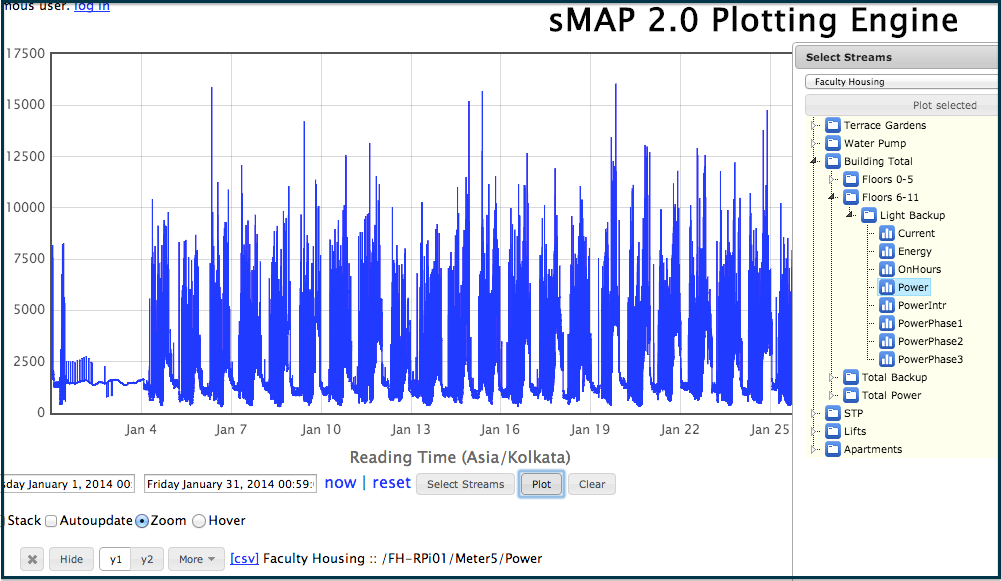
\includegraphics[width=0.8\textwidth,height=0.35\textheight]{screenshot.png}
\caption{Screen shot of the webpage}
\label{fig:screenshot}
\end{figure*}

\item \textbf{ Code } %The implementation of the product of experts model is obtained from Iain Murray's website\footnotemark[\value{http://homepages.inf.ed.ac.uk/imurray2/code/}].
It implements the technique described in Geoff Hinton's paper \cite{hinton2000}. 

\item \textbf{ Time Series :} The time series data of the energy consumption of floor 0 to 5, floor 6 to 11 and total power are plotted below in Figures~\ref{fig:flr05}, ~\ref{fig:flr611}, ~\ref{fig:total}.

\begin{figure*}[t]
\centering
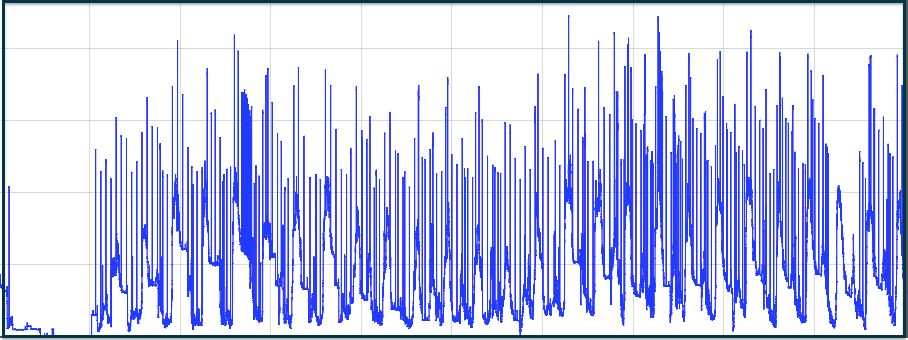
\includegraphics[width=1.0\textwidth,height=0.15\textheight]{floor052.png}
\caption{Stream 1: Power consumption of floors 0-5}
\label{fig:flr05}
\end{figure*}

\begin{figure*}[t]
\centering
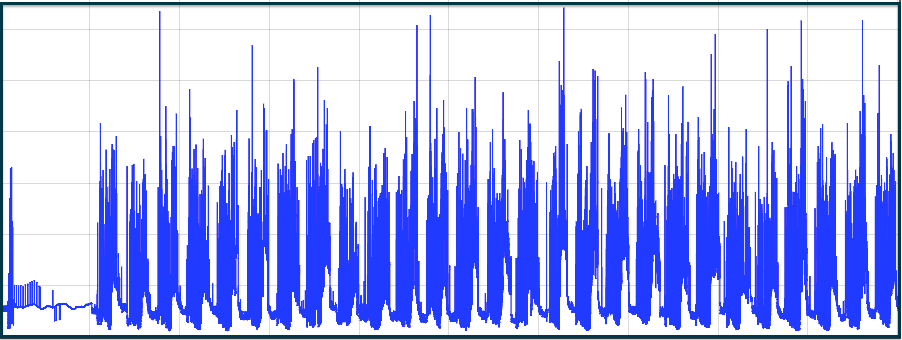
\includegraphics[width=1.0\textwidth,height=0.15\textheight]{floor6112.png}
\caption{Stream 2: Power consumption of floors 6-11}
\label{fig:flr611}
\end{figure*}

\begin{figure*}[th]
\centering
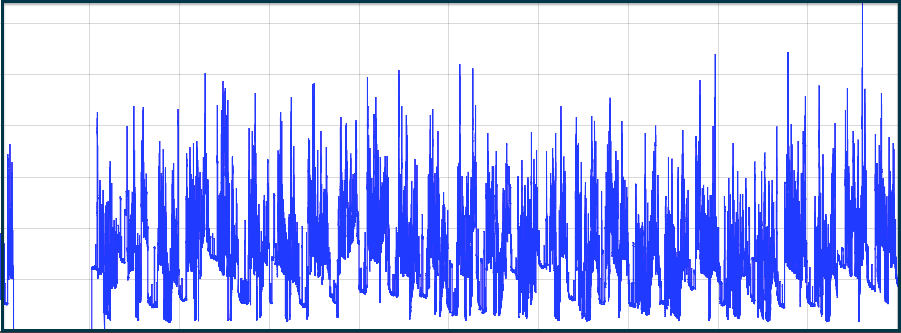
\includegraphics[width=1.0\textwidth,height=0.15\textheight]{total2.png}
\caption{Total Power of the building}
\label{fig:total}
\end{figure*}


\item \textbf{ Additional Details } 
\end{itemize}
\subsection{ Experimental Setup } 
Each of the data stream is modelled as a HMM individually. There are three streams of data, the first stream D$_{1}$ corresponds to the data from 0-5th floor, D$_{2}$ corresponds to 6-11th floor and D$_{3}$ represents the total power from the faculty housing which is represented by a fixed test set, T. Firstly, the stream D$_{1}$ is used to train the model such that the contrastive divergence is minimized. The parameters (mixing component of each unigauss, means of gaussian bits, log precisions of axis-aligned gaussian bits) that are learnt during the training are provided to the test set T in order to obtain the conditional probability of the gaussians given the data D$_{1}$ represented as pgauss$_{1}$. Similarly, the second stream of data, D$_{2}$ collected from floor 6-11, is used to learn the parameters of the model during the training phase which are then again provided to the test set T to obtain conditional probability of the gaussians given the data D$_{2}$ as pgauss$_{2}$. Finally the data D$_{3}$ is used to learn the model and parameters which are then applied to the test set T to obtain the gaussian probability as pgauss$_{3}$. Now, as we know that the total power consumption of the building should be approximately equal to the product of HMMs, which is the product of pgauss$_{1}$ and pgauss$_{2}$. If we can show that the value of pgauss$_{3}$ is as close as possible to the product of pgauss$_{1}$ and pgauss$_{2}$.\\
The experiments performed in table ~\ref{table:error5} , shows the effect of varying samples on KL Divergence, convergence time and iterations keeping minimum threshold constant at 7.\\
The other experiment performed in table ~\ref{table:error6} shows that effect of varying experts on KL Divergence and convergence time.

\subsection{ Results }
Table ~\ref{table:error5} shows that the error was minimum when the sample size was $300$. With respect to the number of experts, the error was minimum when there were $5$ experts as shown in table~\ref{table:error6}.
\begin{table}[htdp]
\begin{center}
\begin{tabular}{| c | c | c | c |}
\hline
Samples & $KL Div$ & $T(sec)$ & $Iterations$ \\
\hline
100 & 2.6219e-05 & 257 & 45100 \\
300 & 1.9753e-05 & 222 & 43200 \\
500 & 5.5493e-05 & 260 & 44800 \\
700 & 3.2847e-05 & 249 & 44000 \\
900 & 3.9486e-04 & 221 & 42600 \\
1100 & 4.9274e-04 & 317 & 44700 \\
1300 & 3.0425e-04 & 276 & 43100 \\
1500 &  3.1128e-04 & 303 & 44400\\
2000 & 1.9192e-04 & 306 & 44400\\
2500 & 1.7122e-04 & 370 & 44100 \\
3000 & 1.4686e-04 & 331 & 43300 \\
3500 & 1.2663e-04 & 370 & 43200 \\
4000 & 1.0793e-04 & 403 & 43200 \\
\hline
\end{tabular}
\end{center}
\caption{Effect of varying samples on KL div}
\label{table:error5}
\end{table}

\begin{table}[htdp]
\begin{center}
\begin{tabular}{| c | c | c |}
\hline
Experts & $KL Div (e-05)$ & $T(sec)$\\
\hline
3 & 1.9780 & 229 \\
4 & 3.5897 & 217 \\
5 & 1.9753 & 228 \\
6 & 4.3488 & 238 \\
7 & 4.9111 & 245  \\
8 & 5.6564 & 241 \\
9 & 5.4290 & 258 \\
10 & 5.5163 & 267 \\
12 & 4.4504 & 262 \\
14 & 6.9006 & 296 \\
16 & 6.8666 & 300 \\
18 & 6.2872 & 313 \\
20 & 5.3842 & 267 \\
25 & 5.8970 & 326 \\
30 & 5.9962 & 327  \\
35 & 5.2716 & 346 \\
40 & 5.0955 & 320 \\
\hline
\end{tabular}
\end{center}
\caption{Effect of varying experts on KL div and time}
\label{table:error6}
\end{table}


%\section{The {\secit Body} of The Paper}
%Typically, the body of a paper is organized
%into a hierarchical structure, with numbered or unnumbered
%headings for sections, subsections, sub-subsections, and even
%smaller sections.  The command \texttt{{\char'134}section} that
%precedes this paragraph is part of such a
%hierarchy.\footnote{This is the second footnote.  It
%starts a series of three footnotes that add nothing
%informational, but just give an idea of how footnotes work
%and look. It is a wordy one, just so you see
%how a longish one plays out.} \LaTeX\ handles the numbering
%and placement of these headings for you, when you use
%the appropriate heading commands around the titles
%of the headings.  If you want a sub-subsection or
%smaller part to be unnumbered in your output, simply append an
%asterisk to the command name.  Examples of both
%numbered and unnumbered headings will appear throughout the
%balance of this sample document.
%
%Because the entire article is contained in
%the \textbf{document} environment, you can indicate the
%start of a new paragraph with a blank line in your
%input file; that is why this sentence forms a separate paragraph.
%
%\subsection{Type Changes and {\subsecit Special} Characters}
%We have already seen several typeface changes in this sample.  You
%can indicate italicized words or phrases in your text with
%the command \texttt{{\char'134}textit}; emboldening with the
%command \texttt{{\char'134}textbf}
%and typewriter-style (for instance, for computer code) with
%\texttt{{\char'134}texttt}.  But remember, you do not
%have to indicate typestyle changes when such changes are
%part of the \textit{structural} elements of your
%article; for instance, the heading of this subsection will
%be in a sans serif\footnote{A third footnote, here.
%Let's make this a rather short one to
%see how it looks.} typeface, but that is handled by the
%document class file. Take care with the use
%of\footnote{A fourth, and last, footnote.}
%the curly braces in typeface changes; they mark
%the beginning and end of
%the text that is to be in the different typeface.
%
%You can use whatever symbols, accented characters, or
%non-English characters you need anywhere in your document;
%you can find a complete list of what is
%available in the \textit{\LaTeX\
%User's Guide}\cite{Lamport:LaTeX}.
%
%\subsection{Math Equations}
%You may want to display math equations in three distinct styles:
%inline, numbered or non-numbered display.  Each of
%the three are discussed in the next sections.
%
%\subsubsection{Inline (In-text) Equations}
%A formula that appears in the running text is called an
%inline or in-text formula.  It is produced by the
%\textbf{math} environment, which can be
%invoked with the usual \texttt{{\char'134}begin. . .{\char'134}end}
%construction or with the short form \texttt{\$. . .\$}. You
%can use any of the symbols and structures,
%from $\alpha$ to $\omega$, available in
%\LaTeX\cite{Lamport:LaTeX}; this section will simply show a
%few examples of in-text equations in context. Notice how
%this equation: \begin{math}\lim_{n\rightarrow \infty}x=0\end{math},
%set here in in-line math style, looks slightly different when
%set in display style.  (See next section).
%
%\subsubsection{Display Equations}
%A numbered display equation -- one set off by vertical space
%from the text and centered horizontally -- is produced
%by the \textbf{equation} environment. An unnumbered display
%equation is produced by the \textbf{displaymath} environment.
%
%Again, in either environment, you can use any of the symbols
%and structures available in \LaTeX; this section will just
%give a couple of examples of display equations in context.
%First, consider the equation, shown as an inline equation above:
%\begin{equation}\lim_{n\rightarrow \infty}x=0\end{equation}
%Notice how it is formatted somewhat differently in
%the \textbf{displaymath}
%environment.  Now, we'll enter an unnumbered equation:
%\begin{displaymath}\sum_{i=0}^{\infty} x + 1\end{displaymath}
%and follow it with another numbered equation:
%\begin{equation}\sum_{i=0}^{\infty}x_i=\int_{0}^{\pi+2} f\end{equation}
%just to demonstrate \LaTeX's able handling of numbering.
%
%\subsection{Citations}
%Citations to articles \cite{bowman:reasoning,
%clark:pct, braams:babel, herlihy:methodology},
%conference proceedings \cite{clark:pct} or
%books \cite{salas:calculus, Lamport:LaTeX} listed
%in the Bibliography section of your
%article will occur throughout the text of your article.
%You should use BibTeX to automatically produce this bibliography;
%you simply need to insert one of several citation commands with
%a key of the item cited in the proper location in
%the \texttt{.tex} file \cite{Lamport:LaTeX}.
%The key is a short reference you invent to uniquely
%identify each work; in this sample document, the key is
%the first author's surname and a
%word from the title.  This identifying key is included
%with each item in the \texttt{.bib} file for your article.
%
%The details of the construction of the \texttt{.bib} file
%are beyond the scope of this sample document, but more
%information can be found in the \textit{Author's Guide},
%and exhaustive details in the \textit{\LaTeX\ User's
%Guide}\cite{Lamport:LaTeX}.
%
%This article shows only the plainest form
%of the citation command, using \texttt{{\char'134}cite}.
%This is what is stipulated in the SIGS style specifications.
%No other citation format is endorsed or supported.
%
%\subsection{Tables}
%Because tables cannot be split across pages, the best
%placement for them is typically the top of the page
%nearest their initial cite.  To
%ensure this proper ``floating'' placement of tables, use the
%environment \textbf{table} to enclose the table's contents and
%the table caption.  The contents of the table itself must go
%in the \textbf{tabular} environment, to
%be aligned properly in rows and columns, with the desired
%horizontal and vertical rules.  Again, detailed instructions
%on \textbf{tabular} material
%is found in the \textit{\LaTeX\ User's Guide}.
%
%Immediately following this sentence is the point at which
%Table 1 is included in the input file; compare the
%placement of the table here with the table in the printed
%dvi output of this document.
%
%\begin{table}
%\centering
%\caption{Frequency of Special Characters}
%\begin{tabular}{|c|c|l|} \hline
%Non-English or Math&Frequency&Comments\\ \hline
%\O & 1 in 1,000& For Swedish names\\ \hline
%$\pi$ & 1 in 5& Common in math\\ \hline
%\$ & 4 in 5 & Used in business\\ \hline
%$\Psi^2_1$ & 1 in 40,000& Unexplained usage\\
%\hline\end{tabular}
%\end{table}
%
%To set a wider table, which takes up the whole width of
%the page's live area, use the environment
%\textbf{table*} to enclose the table's contents and
%the table caption.  As with a single-column table, this wide
%table will ``float" to a location deemed more desirable.
%Immediately following this sentence is the point at which
%Table 2 is included in the input file; again, it is
%instructive to compare the placement of the
%table here with the table in the printed dvi
%output of this document.
%
%
%\begin{table*}
%\centering
%\caption{Some Typical Commands}
%\begin{tabular}{|c|c|l|} \hline
%Command&A Number&Comments\\ \hline
%\texttt{{\char'134}alignauthor} & 100& Author alignment\\ \hline
%\texttt{{\char'134}numberofauthors}& 200& Author enumeration\\ \hline
%\texttt{{\char'134}table}& 300 & For tables\\ \hline
%\texttt{{\char'134}table*}& 400& For wider tables\\ \hline\end{tabular}
%\end{table*}
%% end the environment with {table*}, NOTE not {table}!
%
%\subsection{Figures}
%Like tables, figures cannot be split across pages; the
%best placement for them
%is typically the top or the bottom of the page nearest
%their initial cite.  To ensure this proper ``floating'' placement
%of figures, use the environment
%\textbf{figure} to enclose the figure and its caption.
%
%This sample document contains examples of \textbf{.eps}
%and \textbf{.ps} files to be displayable with \LaTeX.  More
%details on each of these is found in the \textit{Author's Guide}.
%
%%\begin{figure}
%%\centering
%%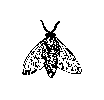
\epsfig{file=fly.eps}
%%\caption{A sample black and white graphic (.eps format).}
%%\end{figure}
%%
%%\begin{figure}
%%\centering
%%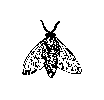
\epsfig{file=fly.eps, height=1in, width=1in}
%%\caption{A sample black and white graphic (.eps format)
%%that has been resized with the \texttt{epsfig} command.}
%%\end{figure}
%
%
%As was the case with tables, you may want a figure
%that spans two columns.  To do this, and still to
%ensure proper ``floating'' placement of tables, use the environment
%\textbf{figure*} to enclose the figure and its caption.
%and don't forget to end the environment with
%{figure*}, not {figure}!
%
%%\begin{figure*}
%%\centering
%%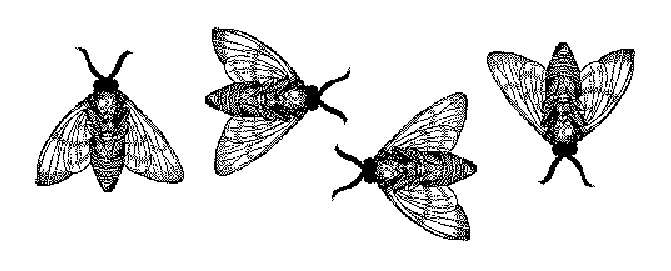
\epsfig{file=flies.eps}
%%\caption{A sample black and white graphic (.eps format)
%%that needs to span two columns of text.}
%%\end{figure*}
%
%Note that either {\textbf{.ps}} or {\textbf{.eps}} formats are
%used; use
%the \texttt{{\char'134}epsfig} or \texttt{{\char'134}psfig}
%commands as appropriate for the different file types.
%
%%\begin{figure}
%%\centering
%%\psfig{file=rosette.ps, height=1in, width=1in,}
%%\caption{A sample black and white graphic (.ps format) that has
%%been resized with the \texttt{psfig} command.}
%%\vskip -6pt
%%\end{figure}
%
%\subsection{Theorem-like Constructs}
%Other common constructs that may occur in your article are
%the forms for logical constructs like theorems, axioms,
%corollaries and proofs.  There are
%two forms, one produced by the
%command \texttt{{\char'134}newtheorem} and the
%other by the command \texttt{{\char'134}newdef}; perhaps
%the clearest and easiest way to distinguish them is
%to compare the two in the output of this sample document:
%
%This uses the \textbf{theorem} environment, created by
%the\linebreak\texttt{{\char'134}newtheorem} command:
%\newtheorem{theorem}{Theorem}
%\begin{theorem}
%Let $f$ be continuous on $[a,b]$.  If $G$ is
%an antiderivative for $f$ on $[a,b]$, then
%\begin{displaymath}\int^b_af(t)dt = G(b) - G(a).\end{displaymath}
%\end{theorem}
%
%The other uses the \textbf{definition} environment, created
%by the \texttt{{\char'134}newdef} command:
%\newdef{definition}{Definition}
%\begin{definition}
%If $z$ is irrational, then by $e^z$ we mean the
%unique number which has
%logarithm $z$: \begin{displaymath}{\log e^z = z}\end{displaymath}
%\end{definition}
%
%Two lists of constructs that use one of these
%forms is given in the
%\textit{Author's  Guidelines}.
% 
%There is one other similar construct environment, which is
%already set up
%for you; i.e. you must \textit{not} use
%a \texttt{{\char'134}newdef} command to
%create it: the \textbf{proof} environment.  Here
%is a example of its use:
%\begin{proof}
%Suppose on the contrary there exists a real number $L$ such that
%\begin{displaymath}
%\lim_{x\rightarrow\infty} \frac{f(x)}{g(x)} = L.
%\end{displaymath}
%Then
%\begin{displaymath}
%l=\lim_{x\rightarrow c} f(x)
%= \lim_{x\rightarrow c}
%\left[ g{x} \cdot \frac{f(x)}{g(x)} \right ]
%= \lim_{x\rightarrow c} g(x) \cdot \lim_{x\rightarrow c}
%\frac{f(x)}{g(x)} = 0\cdot L = 0,
%\end{displaymath}
%which contradicts our assumption that $l\neq 0$.
%\end{proof}
%
%Complete rules about using these environments and using the
%two different creation commands are in the
%\textit{Author's Guide}; please consult it for more
%detailed instructions.  If you need to use another construct,
%not listed therein, which you want to have the same
%formatting as the Theorem
%or the Definition\cite{salas:calculus} shown above,
%use the \texttt{{\char'134}newtheorem} or the
%\texttt{{\char'134}newdef} command,
%respectively, to create it.
%
%\subsection*{A {\secit Caveat} for the \TeX\ Expert}
%Because you have just been given permission to
%use the \texttt{{\char'134}newdef} command to create a
%new form, you might think you can
%use \TeX's \texttt{{\char'134}def} to create a
%new command: \textit{Please refrain from doing this!}
%Remember that your \LaTeX\ source code is primarily intended
%to create camera-ready copy, but may be converted
%to other forms -- e.g. HTML. If you inadvertently omit
%some or all of the \texttt{{\char'134}def}s recompilation will
%be, to say the least, problematic.

\section{Conclusions}
%This paragraph will end the body of this sample document.
%Remember that you might still have Acknowledgments or
%Appendices; brief samples of these
%follow.  There is still the Bibliography to deal with; and
%we will make a disclaimer about that here: with the exception
%of the reference to the \LaTeX\ book, the citations in
%this paper are to articles which have nothing to
%do with the present subject and are used as
%examples only.
%\end{document}  % This is where a 'short' article might terminate

%ACKNOWLEDGMENTS are optional
\section{Acknowledgments}
%This section is optional; it is a location for you
%to acknowledge grants, funding, editing assistance and
%what have you.  In the present case, for example, the
%authors would like to thank Gerald Murray of ACM for
%his help in codifying this \textit{Author's Guide}
%and the \textbf{.cls} and \textbf{.tex} files that it describes.

%
% The following two commands are all you need in the
% initial runs of your .tex file to
% produce the bibliography for the citations in your paper.

%\nocite{Felice,Shen,taban,Albert,wijaya2014consumer,Zhang,Daneshi,bassi,samuel,Falvo,Bakirtzis,Chen,Chow,DisaggregationHSMM,KolterJ12,KolterF11,BLTJ:BLTJ21650,Heinzelman00energy,Taylor,NYAS:NYAS5921,
%Wijaya,5620917,1626400,mckerracher, benveniste,hinton2000,aistats,fhmm,andrew}

%\bibliographystyle{abbrv}
%\bibliography{sigproc}  % sigproc.bib is the name of the Bibliography in this case
% You must have a proper ".bib" file
%  and remember to run:
% latex bibtex latex latex
% to resolve all references
%
% ACM needs 'a single self-contained file'!
%
%APPENDICES are optional
%\balancecolumns
%\appendix
%%Appendix A
%\section{Headings in Appendices}
%The rules about hierarchical headings discussed above for
%the body of the article are different in the appendices.
%In the \textbf{appendix} environment, the command
%\textbf{section} is used to
%indicate the start of each Appendix, with alphabetic order
%designation (i.e. the first is A, the second B, etc.) and
%a title (if you include one).  So, if you need
%hierarchical structure
%\textit{within} an Appendix, start with \textbf{subsection} as the
%highest level. Here is an outline of the body of this
%document in Appendix-appropriate form:
%\subsection{Introduction}
%\subsection{The Body of the Paper}
%\subsubsection{Type Changes and  Special Characters}
%\subsubsection{Math Equations}
%\paragraph{Inline (In-text) Equations}
%\paragraph{Display Equations}
%\subsubsection{Citations}
%\subsubsection{Tables}
%\subsubsection{Figures}
%\subsubsection{Theorem-like Constructs}
%\subsubsection*{A Caveat for the \TeX\ Expert}
%\subsection{Conclusions}
%\subsection{Acknowledgments}
%\subsection{Additional Authors}
%This section is inserted by \LaTeX; you do not insert it.
%You just add the names and information in the
%\texttt{{\char'134}additionalauthors} command at the start
%of the document.

%\subsection{References}
%Generated by bibtex from your ~.bib file.  Run latex,
%then bibtex, then latex twice (to resolve references)
%to create the ~.bbl file.  Insert that ~.bbl file into
%the .tex source file and comment out
%the command \texttt{{\char'134}thebibliography}.

% This next section command marks the start of
% Appendix B, and does not continue the present hierarchy
%\section{More Help for the Hardy}
%The sig-alternate.cls file itself is chock-full of succinct
%and helpful comments.  If you consider yourself a moderately
%experienced to expert user of \LaTeX, you may find reading
%it useful but please remember not to change it.
%\balancecolumns % GM June 2007
% That's all folks!

\nocite{Ghahramani,Felice,Shen,taban,Albert,wijaya2014consumer,Zhang,Daneshi,bassi,samuel,Falvo,Bakirtzis,Chen,Chow,DisaggregationHSMM,KolterJ12,KolterF11,BLTJ:BLTJ21650,Heinzelman00energy,Taylor,NYAS:NYAS5921,
Wijaya,5620917,1626400,mckerracher, benveniste,hinton2000,aistats,fhmm,andrew}


\bibliographystyle{abbrv}
\bibliography{cikm}

\end{document}
